\chapter{Modelo de Despliegue}
\label{modelo_despliegue}

\begin{figure}
 \centering
 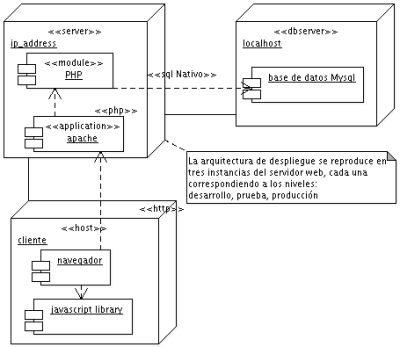
\includegraphics[width=141mm, height=122mm]{despliegue.png}
 \caption{Modelo de Despliegue}
 \label{despliegue}
\end{figure}

El SITEM se despliega sobre un servidor que tenga instalado un programa que acepte peticiones usando el protocolo HTTP - Servidor Web, tenga soporte para el interprete de PHP y un servidor de bases de datos MySQL o PostgreSQL. La figura \ref{despliegue} muestra el diagrama de componentes correspondiente a la arquitectura propuesta.

La arquitectura mostrada se reproduce en tres instancias del servidor web, cada una correspondiendo a los niveles de:

\begin{itemize}
\item \textbf{Desarrollo:} Con las versiones más recientes del sistema que se consideran en versión alfa o inestables. Dentro de la codificación son aquellas que muestran incrementos en el cuarto segmento: AA.XX.YY.\textbf{ZZ}
\item \textbf{Prueba:} Versiones que tienen desarrollos estables pero que aún no han pasado la etapa de revisión de casos de prueba. En la codificación son aquellas que muestran un incremento en el tercer segmento: AA.XX.\textbf{YY}.ZZ 
\item \textbf{Producción:} Versiones que han sido probadas y no tienen errores detectados. De acuerdo a la naturaleza de la funcionalidad alcanzada estas versiones representan un incremento en los segmentos primero o segundo dentro de la codificación. 

Si es el primer segmento el que incrementa se alcanza un ciclo de desarrollo y la versión es bautizada con un nombre específico. Para el SITEM se usan los nombre de los Dioses maya que participaron en alguno de los tres intentos por crear la humanidad.
\end{itemize}
